\documentclass[tikz,border=2pt]{standalone}
\usepackage{amsmath}
\usepackage{pgfplots}
\pgfplotsset{compat=1.18}

\begin{document}
% The identity function returns its input: its graph is the diagonal line y=x, and composing
% any function with it changes nothing.
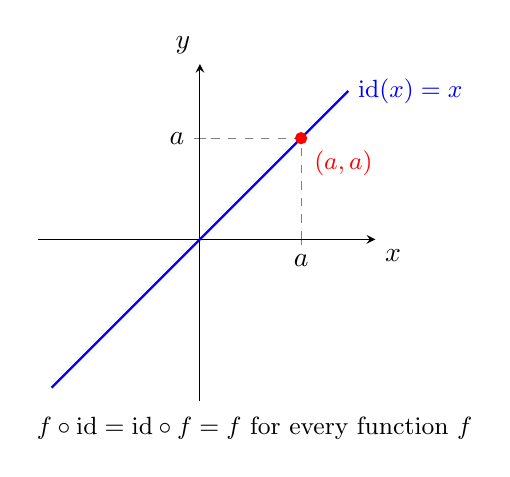
\begin{tikzpicture}
	\begin{axis}[
		axis lines=middle,
		axis equal image,
		xmin=-2.4, xmax=2.6,
		ymin=-2.4, ymax=2.6,
		xtick={1.5}, xticklabels={$a$}, ytick={1.5}, yticklabels={$a$},
		xlabel={$x$}, ylabel={$y$},
		xlabel style={below right}, ylabel style={above left},
		samples=2, clip=false,
		width=6.8cm
		]
		\addplot[thick, blue, domain=-2.2:2.2] {x};
		\addplot[only marks, mark=*, red] coordinates {(1.5,1.5)};
		\draw[dashed, gray] (axis cs:1.5,0) -- (axis cs:1.5,1.5) -- (axis cs:0,1.5);
		\node[blue, anchor=west, font=\small] at (axis cs:2.2,2.2) {$\mathrm{id}(x)=x$};
		\node[red, anchor=north west, font=\small] at (axis cs:1.55,1.45) {$(a,a)$};
	\end{axis}
	\node[anchor=north, font=\small] at ([yshift=-2pt]current axis.outer south) {$f\circ\mathrm{id}=\mathrm{id}\circ f=f$ for every function $f$};
\end{tikzpicture}
\end{document}
